

\section{Experiments and Analysis}

This Section reports the experiments performed to validate our model.
First, we will introduce the ChaLearn dataset, and then present the experimental protocol we followed.
In Section~\ref{sec:results}, we will present and analyse the obtained results, including a discussion
on the modeling elements.
Finally, Section~\ref{sec:ComputationalComplexity} will briefly discuss the computational complexity of the approach.




\subsection{Chalearn LAP Dataset}
\label{sec:chalearn}

%\begin{figure}[t]
%        \centering
%        \begin{subfigure}[c]{.5\textwidth}
%        \centering
%                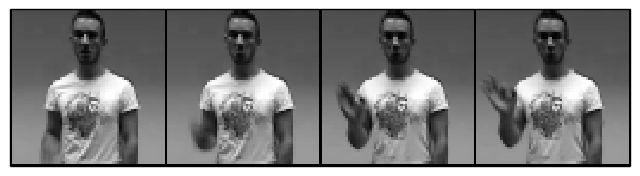
\includegraphics[width=8cm,height=2cm, clip]{images/3dcnn_filters/original_images_gray_body_ok}
%                \caption{``OK"}
%        \end{subfigure}%
%        %
%        \\
%        \begin{subfigure}[c]{0.5\textwidth}
%        \centering
%                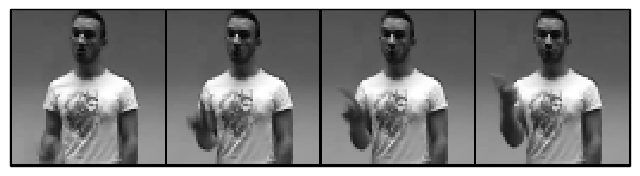
\includegraphics[width=8cm,height=2cm, clip]{images/3dcnn_filters/original_images_gray_body_ncnp}
%                %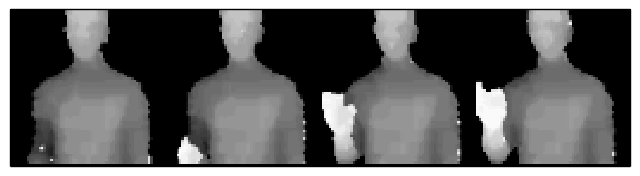
\includegraphics[width=2cm,height=3cm, trim=120 100 100 50, clip]{images/3dcnn_filters/original_images_depth_body_ok}
%                \caption{``Non ce ne piu"}
%        \end{subfigure}
%        \\
%       \begin{subfigure}[c]{0.5\textwidth}
%        \centering
%                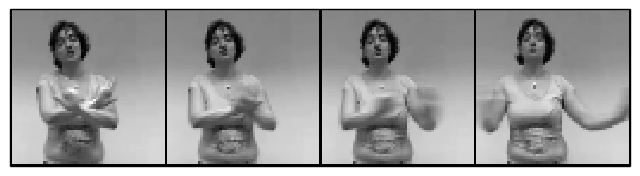
\includegraphics[width=8cm,height=2cm, clip]{images/3dcnn_filters/original_images_gray_body_basta}
%                %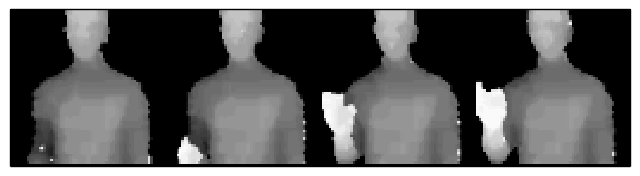
\includegraphics[width=2cm,height=3cm, trim=120 100 100 50, clip]{images/3dcnn_filters/original_images_depth_body_ok}
%                \caption{``Basta"}
%        \end{subfigure}
%       \\
%       \begin{subfigure}[c]{0.5\textwidth}
%        \centering
%                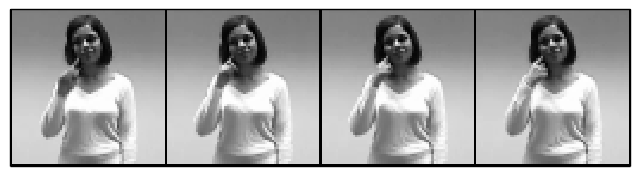
\includegraphics[width=8cm,height=2cm, clip]{images/3dcnn_filters/original_images_gray_body_buonissimo}
%                %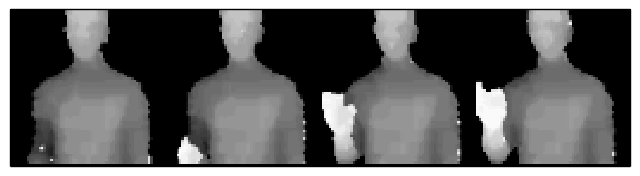
\includegraphics[width=2cm,height=3cm, trim=120 100 100 50, clip]{images/3dcnn_filters/original_images_depth_body_ok}
%                \caption{``Buonissimo"}
%        \end{subfigure}
%               \\
%       \begin{subfigure}[c]{0.5\textwidth}
%        \centering
%                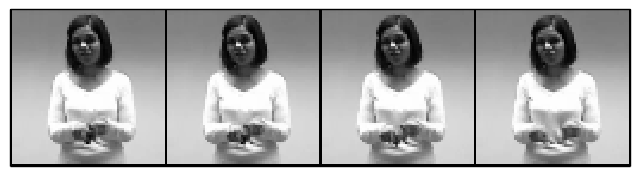
\includegraphics[width=8cm,height=2cm, clip]{images/3dcnn_filters/original_images_gray_body_daccordo}
%                %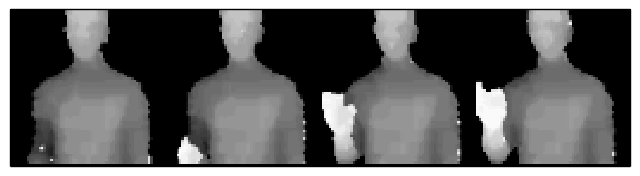
\includegraphics[width=2cm,height=3cm, trim=120 100 100 50, clip]{images/3dcnn_filters/original_images_depth_body_ok}
%                \caption{``Daccordo"}
%        \end{subfigure}
%                       \\
%       \begin{subfigure}[c]{0.5\textwidth}
%        \centering
%                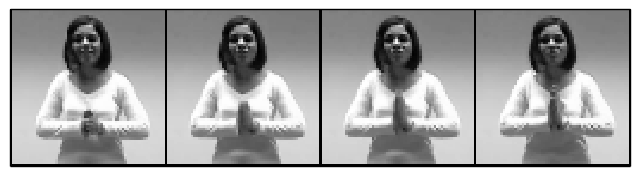
\includegraphics[width=8cm,height=2cm, clip]{images/3dcnn_filters/original_images_gray_body_combinato}
%                %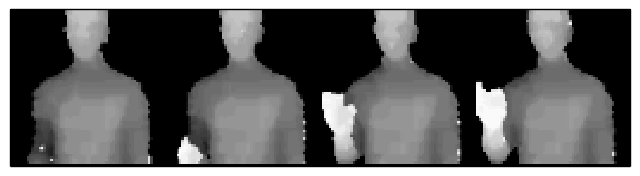
\includegraphics[width=2cm,height=3cm, trim=120 100 100 50, clip]{images/3dcnn_filters/original_images_depth_body_ok}
%                \caption{``Combinato"}
%        \end{subfigure}
%  \caption{
%\mycomline{Add other examples of gestures, interesting to comment upon take them from chalearn website.
%From the confusion matrix, i would propose: ``Basta'', buenissimo, daccordo, combinato}
%\dwucomline{We may not show all the examples here}
%Examples of gestures in the Chalearn dataset.
%Note that some gestures primarily differ primarily in hand pose but not the arm motions, like ``OK'' \emph{vs} ``Non ce ne piu''. ``Basta" and ``Combinato" are the gestures that got mostly misclassified.
%  }
%\label{fig:chalearnclasses}
%\end{figure}






%\mycomline{In this part, provide more information about the dataset: description, content, types of gestures (what are the classes), illustration of the gestures with some pictures (esp. for gestures that have impact on data -for example, expand fig 14 where yoou have the two ok and noncepiu examples with other ones, and put it earlier in the document. why is the dataset challenging ?\\
%Also, provide some statistics about the dataset:
% rough duration of the gestures (average, min max). How many person are performing the gestures, how many occurrences per class, is the dataset balanced}

The dataset used in this work is provided by the ChaLearn LAP \cite{chalearnLAP} gesture spotting challenge\footnote{\href{http://gesture.chalearn.org/2014-looking-at-people-challenge/data-2014-challenge}{http://gesture.chalearn.org/2014-looking-at-people-challenge/data-2014-challenge}}.
%
The focus  is on ``multiple instance, user independent spotting" of gestures, which means learning to recognize gestures from several instances for each category performed by different users, drawn from a gesture vocabulary of 20 Italian cultural/anthropological signs.
A gesture vocabulary is a set of unique gestures, generally related to a particular task.

The challenge dataset contains 940 videos sequences, each performed by a single person and composed of 10 to 20 gesture instances for a total of around $14,000$ gestures.
%
There are 20 gesture classes, \emph{i.e.} \emph{vattene, vieniqui, perfetto, furbo, cheduepalle, chevuoi, daccordo, seipazzo, combinato, freganiente
    , ok, cosatifarei, basta, prendere, noncenepiu, fame, tantotempo, buonissimo, messidaccordo, sonostufo}, with a number a samples well balanced between classes.
% statistics of the gestures here:
The average length of gestures is 39 frames, the minimum frame number for a gesture is 16  and the maximum frame number is 104.

This dataset is challenging because the ``user independent" setting and some of gestures differ primarily in hand pose but not the overall arm motions as illustrated in Fig.~\ref{fig:chalearnclasses}
In terms of data, three modalities are provided with the input videos: the sequence of skeleton joints, and the RGB and depth images
(including a segmentation of the person performing the gesture).
%For the input sequences, there are three modalities provided, \emph{i.e.} skeleton, RGB and depth images (with user segmentation).
% This dataset  is on ``multiple instance, user independent learning and continuous gesture spotting"~\cite{ICMI} of gestures.
% In the 3 track, there are more than 14,000 gestures.

 %\begin{table}[t]
%   \centering
%        \begin{tabular}{|l|c|c|}\hline
%            { Gesture }  &\makebox[5em]{ Length}   &\makebox[5em]{ MAP} \\\hline\hline
%            {\small 1.vattene }            &  38.0   & 0.882  \\\hline
%            {\small 2.vieniqui }           &  36.1   & 0.902  \\\hline
%            {\small 3.perfetto }           &  36.7   & 0.877  \\\hline
%            {\small 4.furbo }              &  40.1   & 0.945  \\\hline
%            {\small 5.cheduepalle }        &  36.9   & 0.949  \\\hline
%            {\small 6.chevuoi }            &  35.9   & 0.926  \\\hline
%            {\small 7.daccordo }           &  40.2   & 0.982  \\\hline
%            {\small 8.seipazzo }           &  43.5   & 0.963  \\\hline
%            {\small 9.combinato }          &  45.6   & 0.956  \\\hline
%            {\small 10.freganiente }        &  37.8   & 0.852  \\\hline
%            %%%%%%%%%%%%%%%%%%%%%%%%%%%%%%%%%%%%%%%%%%
%            {\small 11.ok }                 &  30.8   & 0.778   \\\hline
%            {\small 12.cosatifarei }        &  41.9   & 0.942   \\\hline
%            {\small 13.basta }              &  35.7   & 0.924   \\\hline
%            {\small 14.prendere }           &  37.9   & 0.892   \\\hline
%            {\small 15.noncenepiu }         &  37.5   & 0.774   \\\hline
%            {\small 16.fame }               &  41.3   & 0.958   \\\hline
%            {\small 17.tantotempo }         &  39.1   & 0.955   \\\hline
%            {\small 18.buonissimo }         &  43.5   & 0.905   \\\hline
%            {\small 19.messidaccordo }      &  44.5   & 0.951  \\\hline
%            {\small 20.sonostufo }          &  39.9   & 0.926   \\\hline
%        \end{tabular}
%\vspace*{-2mm}
%    \caption{\dwucomline{Average length of a gesture, this table won't be included in the final version, but just to show to JMO.}
%          }
%          \label{Table_score_fusion}
%\end{table}


\subsection{Experimental protocol}

\setlength{\fboxsep}{1pt}%
\setlength{\fboxrule}{1pt}%
\begin{figure}[t]
       \centering
        \begin{subfigure}[c]{0.15\textwidth}
        \centering
                \fbox{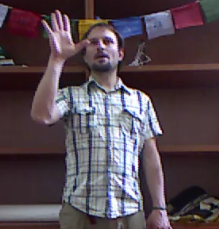
\includegraphics[width=2cm,height=2cm, clip]{images/original/3perfetto.PNG}}
                \caption{\small{``Perfetto"}}
        \end{subfigure}%
        %
        \begin{subfigure}[c]{0.15\textwidth}
        \centering
                \fbox{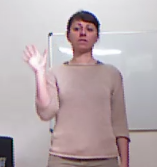
\includegraphics[width=2cm,height=2cm, clip]{images/original/3perfetto2.PNG}}
                %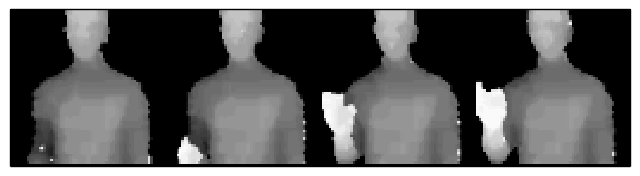
\includegraphics[width=2cm,height=3cm, trim=120 100 100 50, clip]{images/3dcnn_filters/original_images_depth_body_ok}
                \caption{\small{``Perfetto"}}
        \end{subfigure}
       \begin{subfigure}[c]{0.15\textwidth}
        \centering
                \fbox{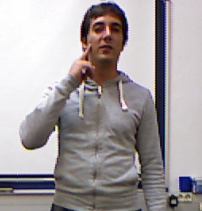
\includegraphics[width=2cm,height=2cm, clip]{images/original/18buonissimo2.PNG}}
                %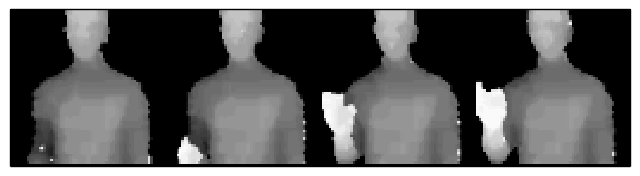
\includegraphics[width=2cm,height=3cm, trim=120 100 100 50, clip]{images/3dcnn_filters/original_images_depth_body_ok}
                \caption{\small{``Buonissimo"}}
        \end{subfigure}
        \\
       \centering
        \begin{subfigure}[c]{0.15\textwidth}
        \centering
                \fbox{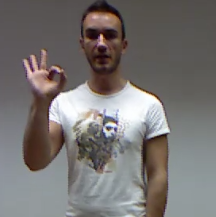
\includegraphics[width=2cm,height=2cm, clip]{images/original/11ok.PNG}}
                \caption{\small{``OK"}}
        \end{subfigure}%
        %
        \begin{subfigure}[c]{0.15\textwidth}
        \centering
                \fbox{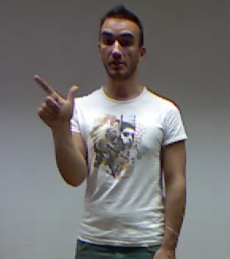
\includegraphics[width=2cm,height=2cm, clip]{images/original/15noncenepiu.PNG}}
                %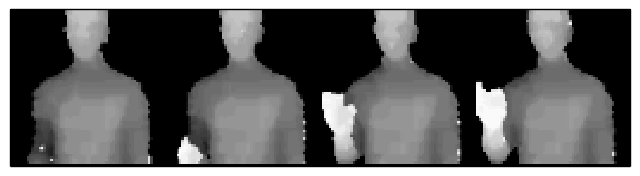
\includegraphics[width=2cm,height=3cm, trim=120 100 100 50, clip]{images/3dcnn_filters/original_images_depth_body_ok}
                \caption{\small{``Non ce ne piu"}}
        \end{subfigure}
       \begin{subfigure}[c]{0.15\textwidth}
        \centering
                \fbox{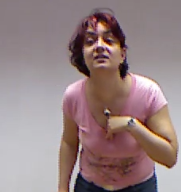
\includegraphics[width=2cm,height=2cm, clip]{images/original/9combinato.PNG}}
                %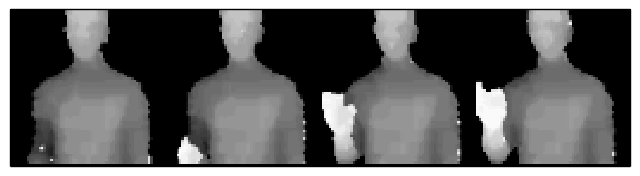
\includegraphics[width=2cm,height=3cm, trim=120 100 100 50, clip]{images/3dcnn_filters/original_images_depth_body_ok}
                \caption{\small{``Combinato"}}
        \end{subfigure}
        \\
            \centering
        \begin{subfigure}[c]{0.15\textwidth}
        \centering
                \fbox{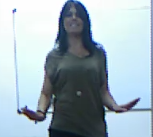
\includegraphics[width=2cm,height=2cm, clip]{images/original/13basta.PNG}}
                \caption{\small{``Basta"}}
        \end{subfigure}%
        %
        \begin{subfigure}[c]{0.15\textwidth}
        \centering
                \fbox{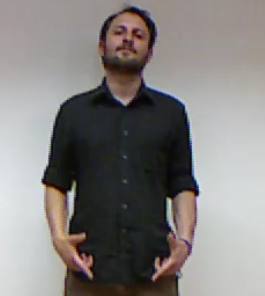
\includegraphics[width=2cm,height=2cm, clip]{images/original/5cheduepalle.PNG}}
                %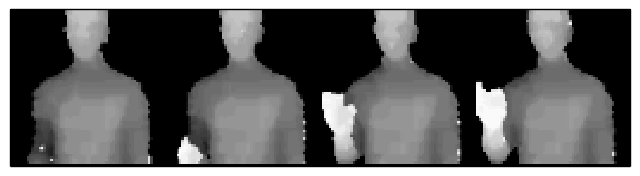
\includegraphics[width=2cm,height=3cm, trim=120 100 100 50, clip]{images/3dcnn_filters/original_images_depth_body_ok}
                \caption{\small{``Cheduepalle"}}
        \end{subfigure}
       \begin{subfigure}[c]{0.15\textwidth}
        \centering
                \fbox{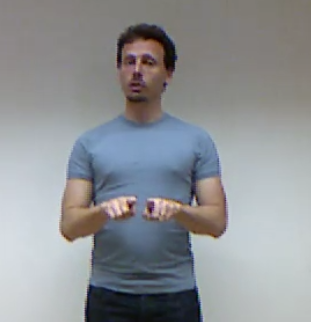
\includegraphics[width=2cm,height=2cm, clip]{images/original/7daccordo.PNG}}
                %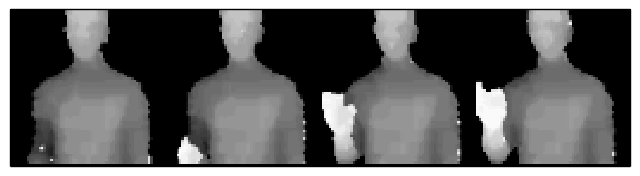
\includegraphics[width=2cm,height=3cm, trim=120 100 100 50, clip]{images/3dcnn_filters/original_images_depth_body_ok}
                \caption{\small{``Daccordo"}}
        \end{subfigure}
  \caption{
%\mycomline{Add other examples of gestures, interesting to comment upon take them from chalearn website.
%From the confusion matrix, i would propose: ``Basta'', buenissimo, daccordo, combinato}
%\dwucomline{We may not show all the examples here}
\small{Examples of gestures in the Chalearn dataset.
This dataset is challenging because the ``user independent" setting (a)\&(b), some of gestures differ primarily in hand pose but not the overall arm motions (d)\&(e) and some gestures require both hands to perform (g,h,i).
Subtle hand movement (c) and differences in performing speed and range (f) also make recognising tasks challenging.
%Note that some gestures primarily differ primarily in hand pose but not the arm motions, like ``OK'' \emph{vs} ``Non ce ne piu''. ``Basta" and ``Combinato" are the gestures that got mostly misclassified.
  }}
\label{fig:chalearnclasses}
\end{figure}
\subsubsection{Training and evaluation protocol}

We follow the ChaLearn experimental protocol, in which the input sequences are split into 700 videos for training, and 240 sequences for testing and reporting results.
Note that the   test sequences  are not segmented a priori and the gestures must be detected within a continuous data stream
which, in addition to the targeted gestures, also contains noisy and out-of-vocabulary gestures.
%
Furthermore, in the experiments, we split the training videos into 650 videos for learning the actual neural network model parameters, and 50 videos
used as validation data for monitoring the training performance or selecting hyper-parameters.


\subsubsection{Performance measures}

Several measures can be used to evaluate the gesture recognition performance.
%
In this work, we adopted the ChaLearn performance measure known as the Jaccard index, which relies on a frame-by-frame prediction accuracy.
More precisely, if $GT_i$ denotes the sequence of ground truth labels in video $i$, and $R_i$ the algorithm output, the Jaccard index
of the video is defined as:
\begin{align}
\jaccardindex_i(GT_i, R_i,g) = \frac{N_s(GT_i, R_i,g)}{N_u(GT_i, R_i,g)},
\\
\mbox{and } \jaccardindex_i = \frac{1}{|{\cal G}_i)|} \sum_{g \in {\cal G}_i} \jaccardindex_i(GT_i, R_i,g)
\end{align}

where $N_s(GT_i, R_i, g)$ denotes the number of frames where the ground truth and result agree on the gesture class $g$,
and $N_u(GT_i, R_i, g)$ denotes the number of frames labeled as a gesture frame $g$ by  either the ground truth or the algorithm,
and ${{\cal G}_i}$ denotes the set of gestures either in the ground truth or detected by the algorithm in sequence $i$\footnote{Note that 'non gesture' frames are thus excluded from the counts.}. The average of the $\jaccardindex_i$ over all test videos is reported as performance measure.
%
Note that experimentally, this measure tends to favours having more false positives than missing true positives, in order to increase the numerator.
%Effective ways to detect false positives should be an interesting aspect of future work.

Being defined at the frame level, the Jaccard index can vary due to variations of the segmentation (both in the ground truth and recognition)
at gesture boundaries, which can be irrelevant from an application viewpoint.
%
Thus, we also defined performance at the gesture event level by following the commonly used PASCAL challenge intersection over union criterion.
More precisely, if for a gesture segment $G$, we have $\frac{G \cap R}{G \cup R} >  0.5$, where R denotes a recognized gesture
segment of the same class, then the  gesture is said to be recognized.
%
If the same relation holds but with a gesture segment of another class, the prediction is incorrect.
Otherwise the gesture is rated as undetected. This allows us to define the \eventaccuracy, \eventconfused and \eventmissed performance measures at the video level,
which are further averaged over test sequences for reporting.


\begin{figure*}[t]
        \centering
        \begin{subfigure}[c]{.85\textwidth}
                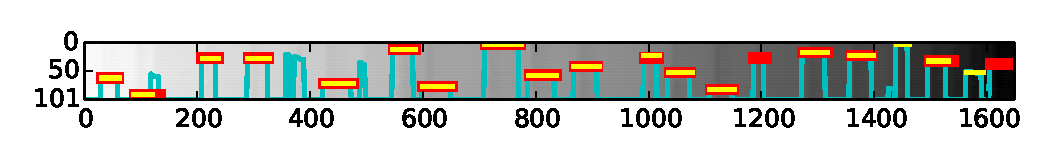
\includegraphics[width=\textwidth]{images/path/Sample0700_sk}
%\vspace*{-3mm}
                \caption{\small{Viterbi decoding from skeleton input.}}
                \label{Sample0700_sk}
        \end{subfigure}%
        ~ %add desired spacing between images, e. g. ~, \quad, \qquad, \hfill etc.
          %(or a blank line to force the subfigure onto a new line)

        \begin{subfigure}[c]{0.85\textwidth}
                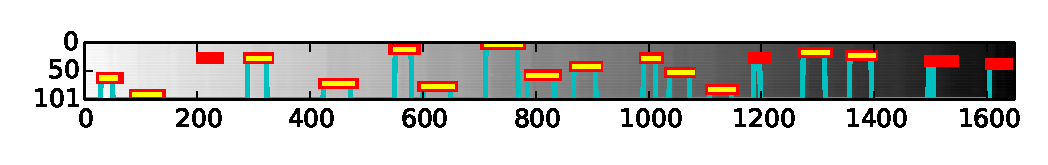
\includegraphics[width=\textwidth]{images/path/Sample0700_cnn}
%\vspace*{-3mm}
                \caption{\small{Viterbi decoding from RGB-D input.}}
                \label{Sample0700_cnn}
        \end{subfigure}

        ~ %add desired spacing between images, e. g. ~, \quad, \qquad, \hfill etc.
          %(or a blank line to force the subfigure onto a new line)
        \begin{subfigure}[c]{0.85\textwidth}
                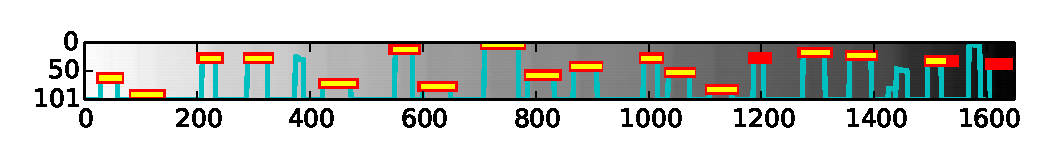
\includegraphics[width=\textwidth]{images/path/Sample0700_combined}
%\vspace*{-3mm}
                \caption{\small{Viterbi decoding from the late fusion of skeleton and RGB-D input.}}
                \label{Sample0700_combined}
        \end{subfigure}
\vspace*{-3mm}
  \caption{
  \small{Viterbi decoding of sample sequence \#700, using skeleton (top), RGB-D (middle) and late fusion system (bottom).
The x-axis represents time and the y-axis represents the hidden states of all classes and of the ergodic state (state $101$).
The cyan lines represent the viterbi shortest path, while red lines denote the ground truth labels,
and the yellow segments  are the predicted labels.
%Two modules exhibit complementary behaviors and generally the skeletal module outperforms the depth module.
The fusion method exploits the complementary properties of individual modules, \emph{e.g.} around frame 200 the skeleton
help solving  the missed detection from the 3DCNN module,
while around frame 1450, the 3DCNN module can help suppress the false positive prediction made by the skeleton module.
}}
\label{fig:Sample0700_comparison}
\end{figure*}

\subsubsection{Tested systems}

We evaluated the recognition performance made by the HMM applied to the emission probabilities estimated from either
the skeleton data, the RGB-D image data, the late fusion scheme, and the intermediate fusion scheme.
%
Note that in all cases the HMM output was further filtered to avoid false alarms,
by considering gesture segments of less than 20 frames as noise and discarding them.
%Note that in all cases the HMM output was further filtered as follows to avoid false alarms.
%First, predicted gesture segments of less than 20 frames were considered as noise and discarded.

%
%% \dwucomline{Actually during the actual test the threshold is set at -inf which does not serve as postprocessing}
%% In addition, longer but noisy gesture segments whose log-probability (including both emission and transition probabilities)  measured over the viterbi path
%% was lower than a threshold were discarded.
%% %
%% This threshold was set by optimizing the Jaccard index on the validation set  of the training data.


%%%%%%%%%%%%%%%%%%%%%%%%%%%%%%%%%%%%%%%%%%%%%%%%%%%%%%%%%%
 \begin{table}[t]
   \centering
        \begin{tabular}{|l||*{2}{c|}}\hline
            {Module }
            &\makebox[5em]{Validation}&\makebox[5em]{Test}
            \\\hline\hline
            {\small Skeleton -- DBDN }            &  0.783    & 0.779 \\\hline
            {\small RGB-D -- 3DCNN }      &  0.752    & 0.717 \\\hline%\hline
            {\small Multimodal Late Fusion }              &  0.817    & 0.809 \\\hline
            {\small Multimodal Inter. Fusion }             &  0.800    & 0.798 \\\hline
        \end{tabular}
\vspace*{-2mm}
    \caption{
    \small{Results in terms of Jaccard index \jaccardindex for the different network structures and modalities modeling the emission probabilities.}
          }
          \label{Table_score_fusion}
          \label{tab:jaccardperformance}
\end{table}
%%%%%%%%%%%%%%%%%%%%%%%%%%%%%%%%%%%%%%%%%%%%%%%%%%%%%%%%%%


%%%%%%%%%%%%%%%%%%%%%%%%%%%%%%%%%%%%%%%%%%%%%%%%%%%%%%%%%%


%%%%%%%%%%%%%%%%%%%%%%%%%%%%%%%%%%%%%%%%%%%%%%%%%%%%%%%%%%

\subsection{Results}\label{sec:results}


%\mycomline{Confusion matrices are fine. However, would it be possible to know the classifiction accuracy of the different classes, for each modality? (i.e the diagonal elements of the confusion matrix? i.e. for instance to look at lowest/highest results? and it improves with fusion?}

\mypartitle{Overall results.}
%
The overal performance of the algorithms are given in Tables~\ref{Table_score_fusion} and~\ref{tab:eventperformance}.
%
As can be observed from both performance measures, the skeleton module usually  performs better than the RGB-D module.
In addition, its generalization capability  is better than that of the RGB-D module,
especially when measured with the Jaccard index where there is almost no drop of performance between the validation and test data.
%
One possible explanation is that the information in the skeleton data is more robust, as it benefited from training using huge and highly
varied data~\cite{shotton2011real}: around on million images from both realistic and synthetic depth images were used to train
the decision forest classifiers involved in the joints extraction.
%
On the over hand, as the  RGB-D module relies on  the raw data and was learned only from the ChaLearn training set, it may
suffer from some overfitting.
%
Another interesting conclusion that can be drawn from Table~\ref{tab:eventperformance} is that while most errors from the RGB-D module are due to under detection
(the \eventmissed rate is 19.7\%, whereas it is only 4.1\% for the skeleton), the skeleton module is more reactive to gesture activity, but makes more mistakes
(the \eventconfused rate is 12.3\% vs 4.5\% for RGB-D).


Finally, the results also demonstrate  that the combination of both modalities is more robust,
as shown by the recognition rate increase and the smaller drop in the generalization performance
%, both at the \jaccardindex and event level
(for instance the decrease of the \eventaccuracy rate is lower than for the skeleton data alone).

 \begin{table}[rt]
   \centering
        \begin{tabular}{|ll||*{2}{c|}}\hline
            %\backslashbox{Module}{Evaluation Set}
             &  \% &  \makebox[3.5em]{Validation}&\makebox[3.5em]{Test}       \\\hline\hline
            \multirow{2}{*}{Skeleton - DBDN}       & \eventaccuracy                & 86.3     & 83.6 \\
                                            &  \eventconfused           & 11.4     & 12.3 \\
                                            &  \eventmissed           &  2.3     &   4.1 \\\hline\hline
            \multirow{2}{*}{RGB-D - 3DCNN}    & \eventaccuracy              & 78.7     & 75.8  \\
                                            &  \eventconfused           & 5.2     &  4.5 \\
                                            &  \eventmissed           & 16.1     & 19.7  \\\hline\hline

            \multirow{2}{*}{Multimodal Late Fusion}   &  \eventaccuracy    & 87.9     & 86.4 \\
                                                      &  \eventconfused    & 9.1     & 8.7 \\
                                                      &  \eventmissed      & 3.0      & 4.9 \\\hline
           \multirow{2}{*}{Multimodal Inter. Fusion}   &  \eventaccuracy    & 86.5     & 85.5\\
                                                      &  \eventconfused    & 7.3      & 6.8 \\
                                                      &  \eventmissed      & 6.2      & 7.7 \\\hline
        \end{tabular}
\vspace*{-2mm}
    \caption{
      \small{ Gesture classification performance at the event level, in percentage of the number of ground truth gestures.}
%\mycomline{table to be finished as for the skeleton}
          }
          \label{tab:eventperformance}
\end{table}

%%%%%%%%%%%%%%%%%%%%%%%%%%%%%%%%%%%%%%%%%%%%%%%%%%%%%%%%%%
\begin{figure}[t]
        \centering
        \begin{subfigure}[c]{.35\textwidth}
                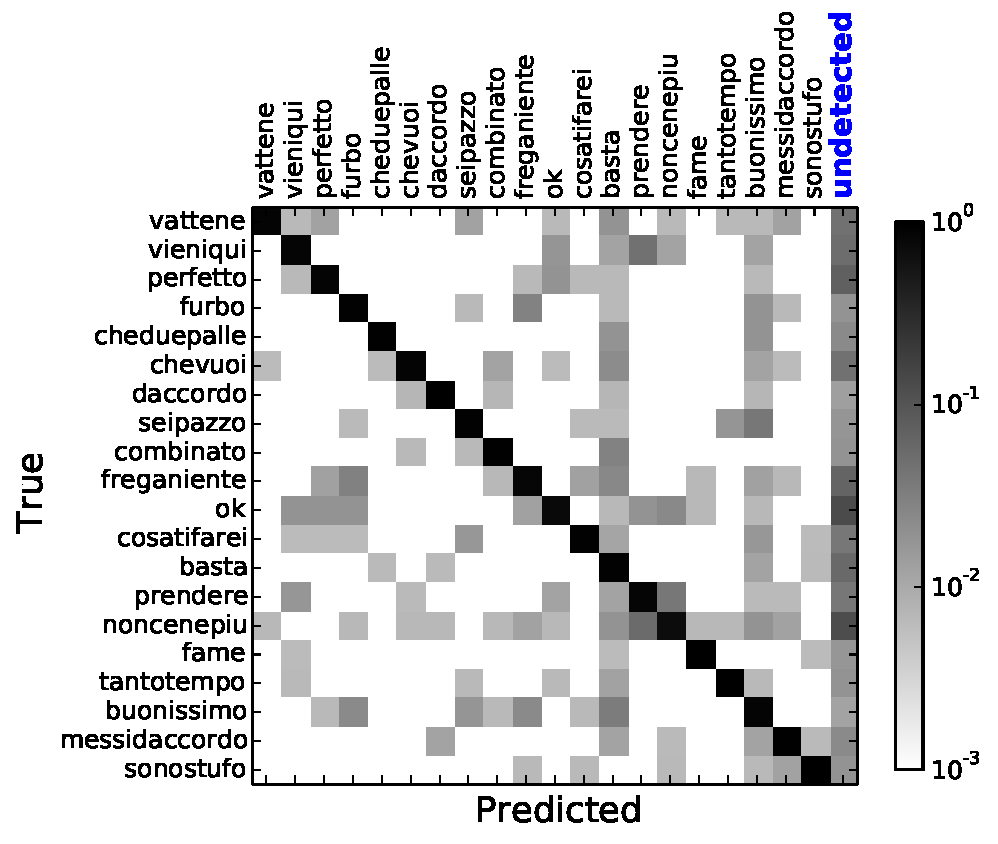
\includegraphics[width=\textwidth]{images/cm/cm_sk}
\vspace*{-3mm}
                \caption{\small{Skeleton - DBN}}
                \label{sk_cm}
        \end{subfigure}%
        ~ %add desired spacing between images, e. g. ~, \quad, \qquad, \hfill etc.
          %(or a blank line to force the subfigure onto a new line)

        \begin{subfigure}[c]{0.35\textwidth}
                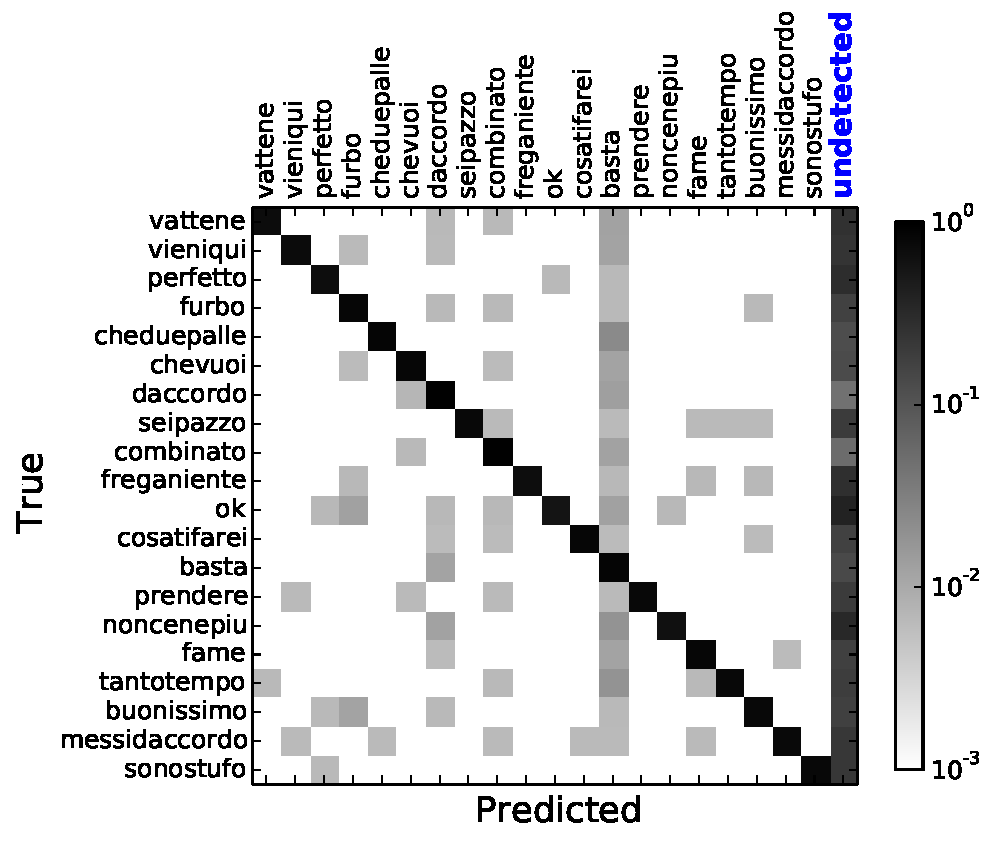
\includegraphics[width=\textwidth]{images/cm/cm_cnn}
\vspace*{-3mm}
                \caption{\small{RGB-D - 3DCNN}}
                \label{cnn_cm}
        \end{subfigure}

        ~ %add desired spacing between images, e. g. ~, \quad, \qquad, \hfill etc.
          %(or a blank line to force the subfigure onto a new line)
        \begin{subfigure}[c]{0.35\textwidth}
                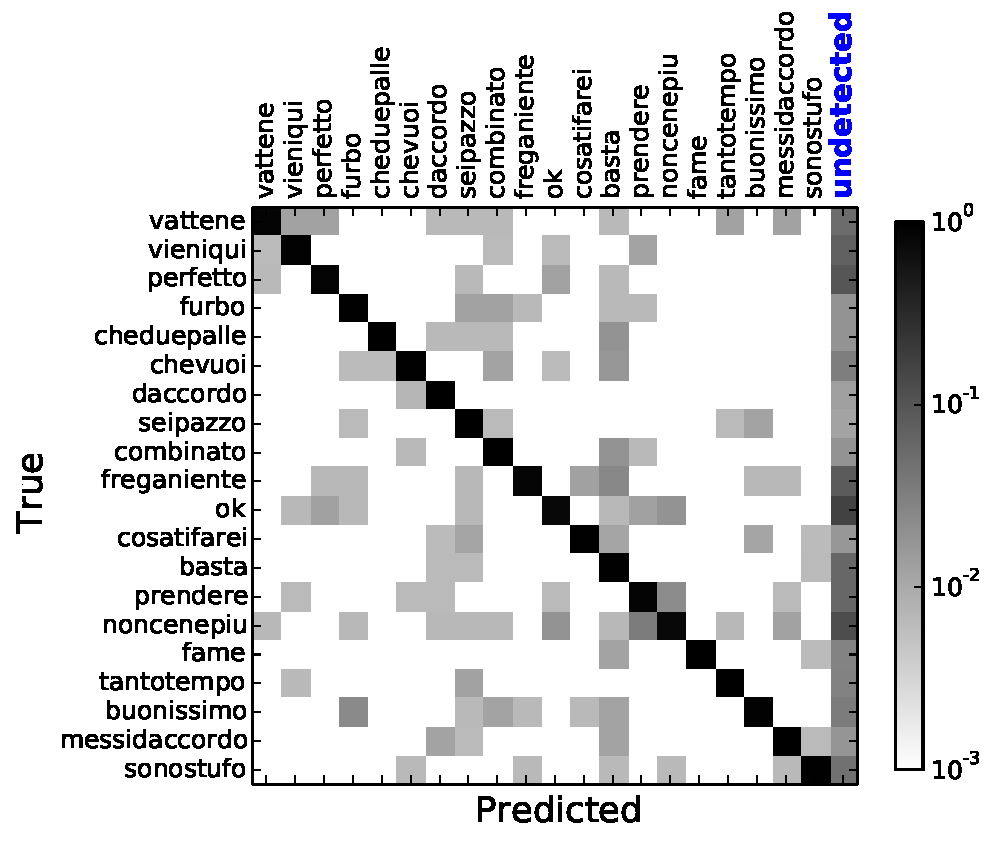
\includegraphics[width=\textwidth]{images/cm/cm_combination}
\vspace*{-3mm}
                \caption{\small{Multimodal Late Fusion}}
                \label{fusion_cm}
        \end{subfigure}

  \caption{\small{Confusion Matrices (log-norm)  for the different modalities.}}
\label{fig:confusion_matrix}
\end{figure}
%%%%%%%%%%%%%%%%%%%%%%%%%%%%%%%%%%%%%%%%%%%%%%%%%%%%%%%%%%

\mypartitle{Confusion matrices.}
%
The confusion matrices (in log-form)
 in Fig.~\ref{fig:confusion_matrix} better illustrate the complementarity of the behaviors of the two modalities.
%
The higher underdetection of RGB-D is clearly visible (whiter matrix, except last 'undetected' column).
%
We can also notice that some gestures are more easily recognized than others,
or catch the difficult instances of other gestures.
This is the case  of the ``Basta" gesture,
whose arms motion  resembles the  start and end of the arm motion of many other gesture (see Fig.~\ref{fig:chalearnclasses}).
Whatever the modality, its model thus tends to recognize few instance of all other gesture classes, whenever their
likelihood are low when being evaluated using the HMM states associated with their true label
due to too much variability.
%
Similarly, the hand movement and pose of the ``Buenissimo" gesture is present in several other gesture classes,
whose instances are then often confused with ``Buenissimo" when relying on the skeleton information alone.
%
However, as these gestures differ primarily in their hand pose, such confusion is much more reduced using the RGB-D domain,
or when fusing  the skeleton and RGB-D modules.
%
The complementary properties of the two modalities is also illustrated from the Viterbi path decoding plot in Fig.~\ref{fig:Sample0700_comparison}.
In general, the benefit of this complementarity between arm pose/gesture and hand pose
can be observed from the whiter confusion matrix than in the skeleton case (less confusion due to hand pose information from RGB-D)
and much less under-detection than in the RGB-D case (better upper-body pose discrimination thanks to skeleton input).
%

However, the modalities by themselves have more difficulties to correct the recognition errors which are due to variations coming from the performer,
like differentiating  people that gesticulate more (see Fig.~\ref{fig:bodydynamics}).

\mypartitle{Late vs. Intermediate  fusion.}
\label{LateIntermediateFusion}
%
The results in Tab.~\ref{tab:jaccardperformance} and~\ref{tab:eventperformance} show that the intermediate fusion system
improved individual modalities, but without outperforming the late fusion system.
%
The result is counter-intuitive, as we would have expected the cross-modality learning in the intermediate fusion scheme
to result in better emission probability predictions, as compared to the simple score fusion in the late system.
%
One possible explanation is that the independence assumption of the late scheme better preserves both
the complementarity and redundancy of the different modalities, properties which are important for fusion.
%
Another related explanation is that in the intermediate fusion learning process,
one modality may dominate and  skew the network towards  learning that specific module and
lowering the importance of the other one.
%
The large difference between the mean activations of the  skeleton module neurons which are predominantly larger than those of the
RGB-D ConvNet's (0.57 \emph{vs.} 0.056) can be an indicator of such a bias during the multimodal fine-tuning phase and
support this conjecture, even if these mean activations are not directly comparable
due to the neuron heterogeneity (the skeleton DBN has logistic units whereas the 3DCNN ConvNet has relu units).
%
Note that such heterogeneity was not present when fusing modalities  in \cite{Ngiam2011multimodal},
where better registration and less spatial registration variability in lip images
allowed to also resort to the same stacked RBMs for the visual modality (rather than \ThreeDCNN)  and the audio one.
%
More investigation on how to handle heterogeneous networks  should be conducted.



%\mycomline{In this comment on the results and benefit of the temporal model, as we discussed.}
%

\mypartitle{HMM benefit.}
%
As the emission probabilities are learned in a discriminative manner, one could  wonder whether the HMM brings benefit beyond smoothing.
To investigate this issue, we removed the temporal structure as follows:
for a given gesture \gesturea, we computed its score at time $t$, $Score(\gesturea,t)$, by summing the emission
log-probabilities $p(\observation_t|\hiddenstate_t = \hiddenstatenode)$ for all nodes associated to that gesture,
\ie $\hiddenstatenode \in \finiteset_{\gesturea}$.
%
This score is then smoothed in the temporal domain (using a window of 5 frames) to obtain $\widehat{Score}(\gesturea,t)$.
%
Finally, following \cite{neverova2014moddrop}, the gesture recognition proceeds in two steps:
first finding gesture segments by thresholding the score of the ergodic state;
then, for each resulting gesture segment, the recognized gesture is defined as the one whose average score within the segment is the highest.
%
Fig.~\ref{fig:temporalModellingComparision} illustrates this process along with the DDNN and ground-truth.
%\mycomline{The figure should show the procedure described above, that you used. It should also illustrate why the jaccard index is so low.}
%\mycomline{``Without temporal modelling, the decision boundary of a gesture will be more rugged and it is
%more difficult to make hard decisions of where the gesture starts or ends.'': is the very low jaccard index just a problem of
%having errors on the event boudary? that sounds strange to me (and would not be a so strong argument;
%in that case the event measure should be computed to check this.}
%
%\dwucomline{No temporal modelling:
%
%To investigate the benefit of temporal modelling of the proposed system, we compare the model that discards temporal modelling. Specially, once, we collect the emission probability \emissionprob{}, we average the hidden states for each gesture class and obtain the frame based gesture class prediction \gestureEmissionProb where \gesturehiddenstateFrame denotes the gesture variables. After temporal smoothing for each frame, a threshold for cutting the begin and end of active gesture is chosen by a validation set. Fig.~\ref{fig:temporalModellingComparision} illustrates the effect of temporal modelling.
The decision boundary of where the gesture starts and ends in the proposed \emph{DDNN} is clean-cut due to the state-diagram defined in Fig.~\ref{HMM_ES}. And the overall performance in terms of  Jaccard index is reduced to $0.660$ for test set.
The \emph{Recognized}, \emph{Confused} and \emph{Missed} correspond to Table~\ref{tab:eventperformance} for test set are  $76.6$ , $5.3$ and $18.1$. The increased miss detection rate reinforces the importance of temporal modelling for better deciding gesture boundary.
 Note that, this representation learning template matching method using only 5 frames still outperforms the Jaccard index $0.413$ using 5 frames template matching system in~\cite{camgoz2014gesture} where all the features are handcrafted.

%% To investigate the benefit of temporal modelling of the proposed system, we compare the model that discards temporal modelling. Specially, once, we collect the emission probability \emissionprob{}, we average the hidden states for each gesture class and obtain the frame based gesture class prediction \gestureEmissionProb where \gesturehiddenstateFrame denotes the gesture variables. After temporal smoothing for each frame, a threshold for cutting the begin and end of active gesture is chosen by a validation set. Fig.~\ref{fig:temporalModellingComparision} illustrates the effect of temporal modelling. The decision boundary of where the gesture starts and ends in the proposed \emph{DDNN} is clean-cut due to the state-diagram defined in Fig.~\ref{HMM_ES}.
%% %
%% And the overall performance in terms of  Jaccard index is reduced to $0.535$ for test set.
%% Note that, this representation learning template matching method using only 5 frames still outperforms
%% the Jaccard index $0.413$ in~\cite{camgoz2014gesture} where all the features are handcrafted.




\mypartitle{Comparison with the state-of-the-art.}
The performance of recent state-of-the-art techniques is given in Table~\ref{tab:soa}. The first half of the table resort to hand crafted feature approaches and then usually a second stage classifier. Our proposed system performs on par with the top two methods. However, hand crafted feature methods' performance is saturated regardless of the increase training data. The representation learning methods in the second half of the Table perform comparably with the best hand crafted feature approaches and the top representation method achieves the best Jaccard index score. Given more training data, it's expected the networks will be able to be more adapted to this ``user independent" setting and learn user invariant features in a transfer learning fashion. It also worths noting that our proposed system is the only method that incorporates the temporal modelling element rather than sliding window approach. We believe this is an interesting research direction that can be more adapted to various lengths of gestures and relevant temporal factors.

%\mypartitle{Comparison with the state-of-the-art. In particular, add discussion that other temporal module could be used,
%including those that could lead to the training of a full deep-neural network.  }
%


\begin{figure*}[t]
  \centering
  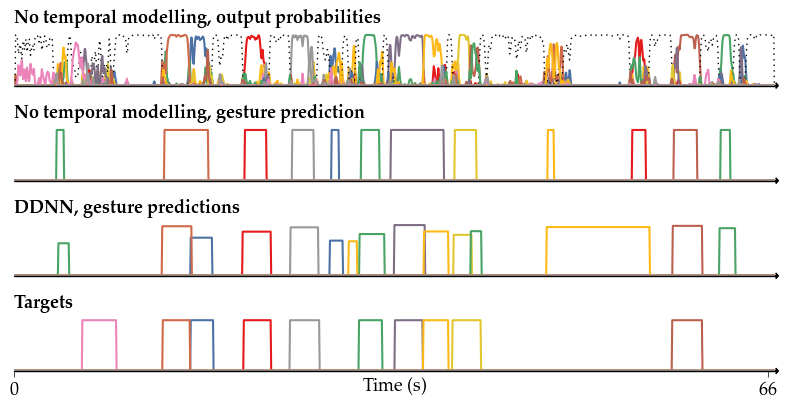
\includegraphics[width=.7\textwidth]{images/output.png}
  \caption{
  \small{The output probabilities are shown for a sequence fragment for the test set \#703. The dashed line represents silence and different colour represent different gestures. Without temporal modelling, the decision boundary of a gesture will be more rugged and it is more difficult to make hard decisions of where the gesture starts or ends. Hence, it causes miss-detection and miss-merging. Because of the temporal modelling and Viterbi path decoding, the gesture boundary will have a clean jump from the ergodic state to the gesture states, resembling the behavior of the manual annotators with better accuracy.}}
    \label{fig:temporalModellingComparision}
\end{figure*}

%%%%%%%%%%%%%%%%%%%%%%%%%%%%%%%%%%%%%%%%%%%%%%%%%%%%%%%%%%

\begin{figure}[t]
        \centering
        \begin{subfigure}[c]{.5\textwidth}
        \centering
                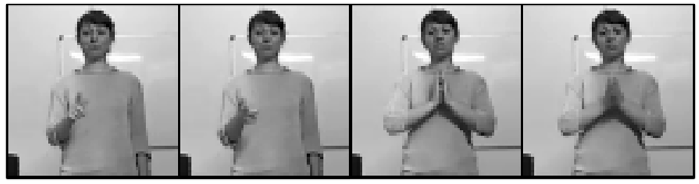
\includegraphics[width=8cm,height=2cm, clip]{images/original806.png}
                \caption{\small{Sample \#806}}
        \end{subfigure}%
        %
        \\
        \begin{subfigure}[c]{0.5\textwidth}
        \centering
                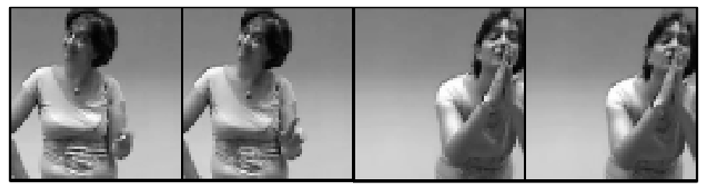
\includegraphics[width=8cm,height=2cm, clip]{images/original702.png}
                %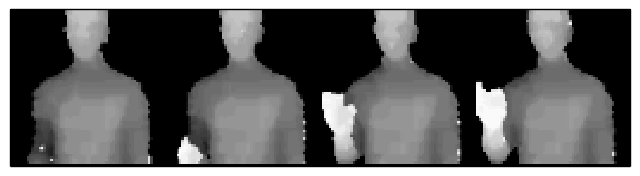
\includegraphics[width=2cm,height=3cm, trim=120 100 100 50, clip]{images/3dcnn_filters/original_images_depth_body_ok}
                \caption{\small{Sample \#702}}
        \end{subfigure}

  \caption{
\small{Examples of performer variations in the  upper body dynamic.
Using \emph{DDNN} (late fusion), Jaccard index of top is 0.95 while bottom is only 0.61.
While most performers tend to keep their upper-body static while performing the gesture, leading to good recognition performance. Vehemently moving of the body when doing the gestures, could make the gestures harder to be recognised.}
  }
\label{fig:bodydynamics}
\end{figure}



%%%%%%%%%%%%%%%%%%%%%%%%%%%%%%%%%%%%%%%%%%%%%%%%%%%%%%%%%%%%
 \begin{table}[t]
   \centering
        \begin{tabular}{|l||*{3}{c|}}\hline
            \makebox[4em]{Module}
            &\makebox[2em]{Skeleton}&\makebox[2em]{RGB-D}&\makebox[2em]{Fusion}
            \\\hline\hline

            {~\cite{Monnier2014multi}} {\scriptsize 3 set skeletal \& HOG, Boosted classifier}                    &  0.791     & -           & 0.822 \\\hline
            {~\cite{Chang2014multi}}  {\scriptsize 3D skeletal pose \& HOG, MRF }            &  0.790& -        & 0.827\\\hline
            {~\cite{Peng2014multi}}  {\scriptsize  Dense trajectory (HOG, HOF, MBH)  }                       &  -         &0.792& - \\\hline
            {~\cite{camgoz2014gesture}} {\scriptsize Template based Random Forest Classifier} &      -     &      -       & 0.747    \\\hline
            {~\cite{evangelidis2014continuous}} {\scriptsize Fisher Vector, Dynamic Programming} &      0.745     &      -       & -  \\\hline
            {~\cite{chen2014multi}} {\scriptsize Independent Subspace Analysis, RF } &      -     &      0.649       & -    \\\hline
            {~\cite{liang2014multi}} {\scriptsize PHOG, SVM, HMM } &      0.454    &      0.462       & 0.597
            \\\hline\hline

            %{~\cite{neverova2014multi}} {\scriptsize Representation Learning (Step 4)        }           &  0.789     & 0.799      & \textbf{0.845}\\\hline
            {~\cite{neverova2014multi}} {\scriptsize Representation Learning (multiscal)  }              &  0.808     & 0.809      & \textbf{ 0.849}\\\hline
            {~\cite{lio2014deep}}     {\scriptsize CNN             }                          &  -         & 0.789      & - \\\hline
            {~\cite{wu2014deep}}   {\scriptsize Deep Neural Networks       }                         &  0.747     & 0.637      & 0.804
            \\\hline\hline
            \textbf{\emph{DDNN}} (this work)                                    &  0.779     & 0.717      & 0.809\\\hline
        \end{tabular}
    \caption{
%\mycomline{Add one or two worse results; separate hand crafted features from neural net methods.}
   \small{ Comparison of results in terms of the ChaLearn Jaccard index with state-of-the-art related works.}
          }
          \label{tab:soa}
\end{table}


\subsection{Computational Complexity}
\label{sec:ComputationalComplexity}

We can distinguish between two complexities: the training one, and the test one.

\mypartitle{Complexity at training time.}
%
Although training deep neural network using stochastic gradient descent is computationally intensive,
the reuse of pre-trained network parameters as done in our case can help with  better initialisation and lead  to faster convergence.
%
We can observe different training time in function of the modality (and architecture).
%
Specifically, using a modern GPU (GeForece GTX TITAN Black) and conv op. by Theano~\cite{Bastien-Theano-2012},
the training time of each epoch of the DBN skeleton module is less than 300 seconds and allows training the required 500 epochs within 2 days.
%
The training time of each epoch of the 3DCNN \RGBD  module is much more  expensive,
taking more than 10,000 seconds.
Hence, 40 epochs takes around 5 days to train.
%
The fusion network being initialised with the individual module parameters, its training time is half that of the 3DCNN.


\mypartitle{Complexity at test time.}
%
Given the learned models, our framework with the above GPU can perform real-time video sequence labelling with a low inference cost.
%
More specifically, a single feed forward neural network incurs linear computational time ($\mathcal{O}(T)$),
and is efficient because it requires only matrix products and convolution operations.
The complexity of the Viterbi algorithm is itself of $\mathcal{O} (T* |S|^2)$, where
$T$ is the number of frames and $|S|$ the number of states, and thus performs real-time given our state-space.
In practice, our multimodal neural network can be deployed at 90 FPS.
The preprocessing part takes most of the time and our un-optimized version runs at 25 FPS, while the
 Viterbi decoding  runs at 90 FPS. Hence, the overall system can achieve faster than real-time performance.


\endinput
